%%%% CAPÍTULO 1 - INTRODUÇÃO
%%
%% Deve apresentar uma visão global da pesquisa, incluindo: breve histórico, importância e justificativa da escolha do tema,
%% delimitações do assunto, formulação de hipóteses e objetivos da pesquisa e estrutura do trabalho.

%% Título e rótulo de capítulo (rótulos não devem conter caracteres especiais, acentuados ou cedilha)
\chapter{Introdução}\label{cap:introducao}

Desde o nascimento, os seres humanos desenvolvem capacidades de reconhecimento e 
identificação de objetos, onde essa capacidade foi muito 
importante durante o processo evolutivo da espécie humana. Sendo as primeiras 
demonstrações de identificação de seres vivos e objetos, datados no período 
pré-histórico.

A biometria, do grego \textit{bios}-vida e \textit{metron}-medida, pode ser 
definida como o processo de identificação de aspectos físicos, biológicos e até 
comportamentais dos seres vivos. Na qual, são utilizados para distinguir indivíduos, 
a partir de suas características únicas. Como por exemplo, a face, retina, 
íris, impressões digitais, geometria da mão, etc.

Dentre as tecnologias atuais de segurança, a biometria tem sido amplamente 
utilizada, seja para acessar contas bancárias, aplicativos e até controlar 
o acesso a locais públicos e privados. Atualmente o reconhecimento facial 
é uma das biometrias mais estudadas, pois além da praticidade é considerada uma 
das formas mais seguras de identificação. 

Embora seja promissora, mesmo assim, o sistema de identificação pode falhar durante o 
processo de reconhecimento, principalmente devido a equívocos e interpretações 
incorretas do \textit{software}. Esses problemas podem ser causados,
desde sujeira na lente da câmera, alta umidade, baixa iluminação, filtros digitais 
não calibrados, ruídos, excesso de informação, inserção de dados falsos, etc.

Desta forma, para um sistema biométrico obter uma alta assertividade, 
deve-se validar todos os cenários possíveis e tomar os devidos cuidados durante seu 
desenvolvimento. Pois, por exemplo, durante o processo de reconhecimento facial,
pode-se haver falsos-positivo ou verdadeiros-negativo (\autoref{fig:pareidolia}), 
ou seja, o \textit{software} pode identificar um rosto humano que não existe, 
ou não identificar um rosto humano, mesmo existindo.

\begin{figure}[h!]
    \centering
    \caption{Imagens que lembram rostos humanos}
    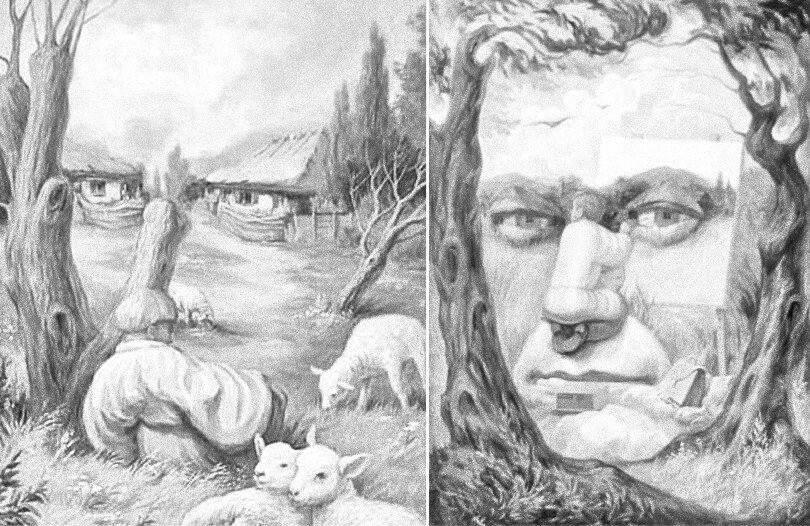
\includegraphics[scale=0.25]{figuras/pareidolia.jpg} 
    \legend{Fonte: Adaptado de \citeonline{pareidoliaimg}.}
    \label{fig:pareidolia}
    \centering
\end{figure}

Como solução, as literaturas recentes propõem novas técnicas de visão computacional, 
reconhecimento e aprendizado de máquina. Em razão disso, a taxa de assertividade 
vem aumentando, devido ao progresso dos sistemas computacionais e dos 
novos \textit{hardwares}, sendo possível obter um maior desempenho, com um custo
menor.

Diante disso, o presente estudo visa discorrer sobre o desenvolvimento de um protótipo 
para o controle de acesso, utilizando reconhecimento facial com SBC e OPENCV.

\section{Objetivos}\label{sec:objetivos}

Neste capítulo serão apresentados os objetivos deste trabalho e as etapas necessárias 
para o desenvolvimento do protótipo. Na qual, além da implementação do 
\textit{hardware}, também serão necessárias algumas etapas para a elaboração do \textit{software}, 
tendo como finalidade, obter uma alta assertividade no controle de acesso por 
reconhecimento facial.

\subsection{Objetivo geral}\label{subsec:objetivoGeral}

Este trabalho tem por objetivo realizar o estudo e desenvolvimento de um protótipo 
para controle de acesso por meio de reconhecimento facial. Para isso, serão implementados 
algorítimos de visão computacional e aprendizado de maquina, em um computador de placa 
única (ESP32-CAM).

\subsection{Objetivos específicos}\label{subsec:objetivosEspecificos}

Para que se cumpram os objetivos gerais, serão essenciais a realização de algumas etapas, 
as quais, são apresentadas a seguir:

\begin{itemize}
    \item  Desenvolver o \textit{hardware} para aquisição de imagens, levando em 
    consideração a luminosidade local e a qualidade da câmera. Garantindo assim, 
    bons resultados para a etapa de reconhecimento facial.
  
    \item Implementar um código que seja otimizado e organizado, o suficiente para 
    conseguir filtrar e processar as imagens em quase tempo real. 
    
    \item Desenvolver uma interface física, onde os usuários possam interagir e 
    utilizar de forma simples e prática.
    
    \item Por último, criar um sistema para controle de acesso, onde o usuário 
    administrador, poderá gerenciar e cadastrar novos usuários, permitindo ou 
    restringindo o acesso, conforme necessário. 
\end{itemize}

\section{Justificativa}\label{sec:justificativa}

Os sistemas de reconhecimento facial foram uma grande solução durante a retomada 
das atividades presenciais após a pandemia do coronavírus, ajudando empresas
a promoverem uma maior segurança física, como também segurança sanitária, 
evitando contaminações e agilizando os processos. Ao contrário dos sistemas 
manuais, onde normalmente geram atrasos e demandam atenção.

Atualmente o controle de acesso mais comum, são aqueles que utilizam chaves 
e tags, porém, como possuem inúmeras fragilidades, estes procedimentos não são 
recomendados em locais que recebem um grande fluxo de pessoas, como por exemplo, 
hotéis e centros comerciais. Pois, desta forma, qualquer pessoa pode ter acesso, 
sem necessariamente estar credenciada.

Outro ponto importante é que a implantação de sistemas automatizados, também 
podem gerar economias. Como por exemplo, em condomínios e hotéis, onde o 
sistema pode realizar parte do serviço de porteiros e/ou recepcionistas, 
possibilitando uma redução na carga horária destes trabalhadores e 
inclusive, resultando na redução de custos para as empresas.

Por fim, a facilidade desses sistemas, fazem com que os usuários não precisem 
mais memorizar senhas, ou carregar suas chaves, impactando positivamente na 
experiência de uso. Além disso, esse sistema reduz a probabilidade de golpes 
ou fraudes, pois impossibilita o compartilhamento do mesmo acesso.

\section{Cronograma}\label{sec:cronograma}

O cronograma abaixo (\autoref{quad:quadro1}), mostra as atividades que 
serão realizadas durante o desenvolvimento deste trabalho.

\begin{tabframed}[htb]
    \caption{Cronograma de desenvolvimento do trabalho}
    \label{quad:quadro1}
    \begin{tabular}{|l|*{12}{p{0.04\textwidth-\columnsep}|}}
    \hline
    \multirow{2}{*}{\textbf{Etapa}} & \multicolumn{5}{c|}{\textbf{2022}} & \multicolumn{6}{c|}{\textbf{2023}} \\  
    \cline{2-12}
    &\textbf{Ag} &\textbf{Se} &\textbf{Ou} &\textbf{No} &\textbf{De} &\textbf{Ja} &\textbf{Fe} &\textbf{Ma} &\textbf{Ab} &\textbf{Ma} &\textbf{Ju} \\ \hline
    Definição do tema                                 &X & & & & & & & & & & \\   \hline
    Definição do escopo do trabalho                   &X & & & & & & & & & & \\   \hline
    Analise de viabilidade e planejamento da execução &X & & & & & & & & & & \\   \hline
    Revisão Bibliográfica                             & &X &X &X & & & & & & & \\ \hline
    Pesquisa sobre ESP32-CAM e OpenCV                     & &X &X & & & & & & & & \\  \hline
    Estudo da plataforma Nextion Editor               & & & &X &X & & & & & & \\  \hline
    Desenvolvimento do protótipo                      & & & & &X &X &X & & & & \\ \hline
    Aplicação do reconhecimento facial                & & & & & &X &X & & & & \\  \hline
    Análise dos resultados                            & & & & & & &X &X & & & \\  \hline
    Correção de erros e aprimoramentos                & & & & & & & &X &X &X & \\ \hline
    Escrita do trabalho                               &X &X &X &X &X &X &X &X &X &X &X \\ \hline
    Apresentação do trabalho                          & & & & & & & & & & &X \\   \hline
    \end{tabular}
    \fonte{}%% Fonte
\end{tabframed}
